This event facilitates generating a CFD model for wind flow around a building. A template is provided to the user to generate an OpenFOAM model based on a set of parameters for mesh generation and CFD simulation. The user needs to specify the domain size, mesh size, boundary conditions, simulation parameters and the method for extracting wind forces on the building as shown in \Cref{fig:cfd_template}.

\begin{figure}[!htbp]
    \centering {
        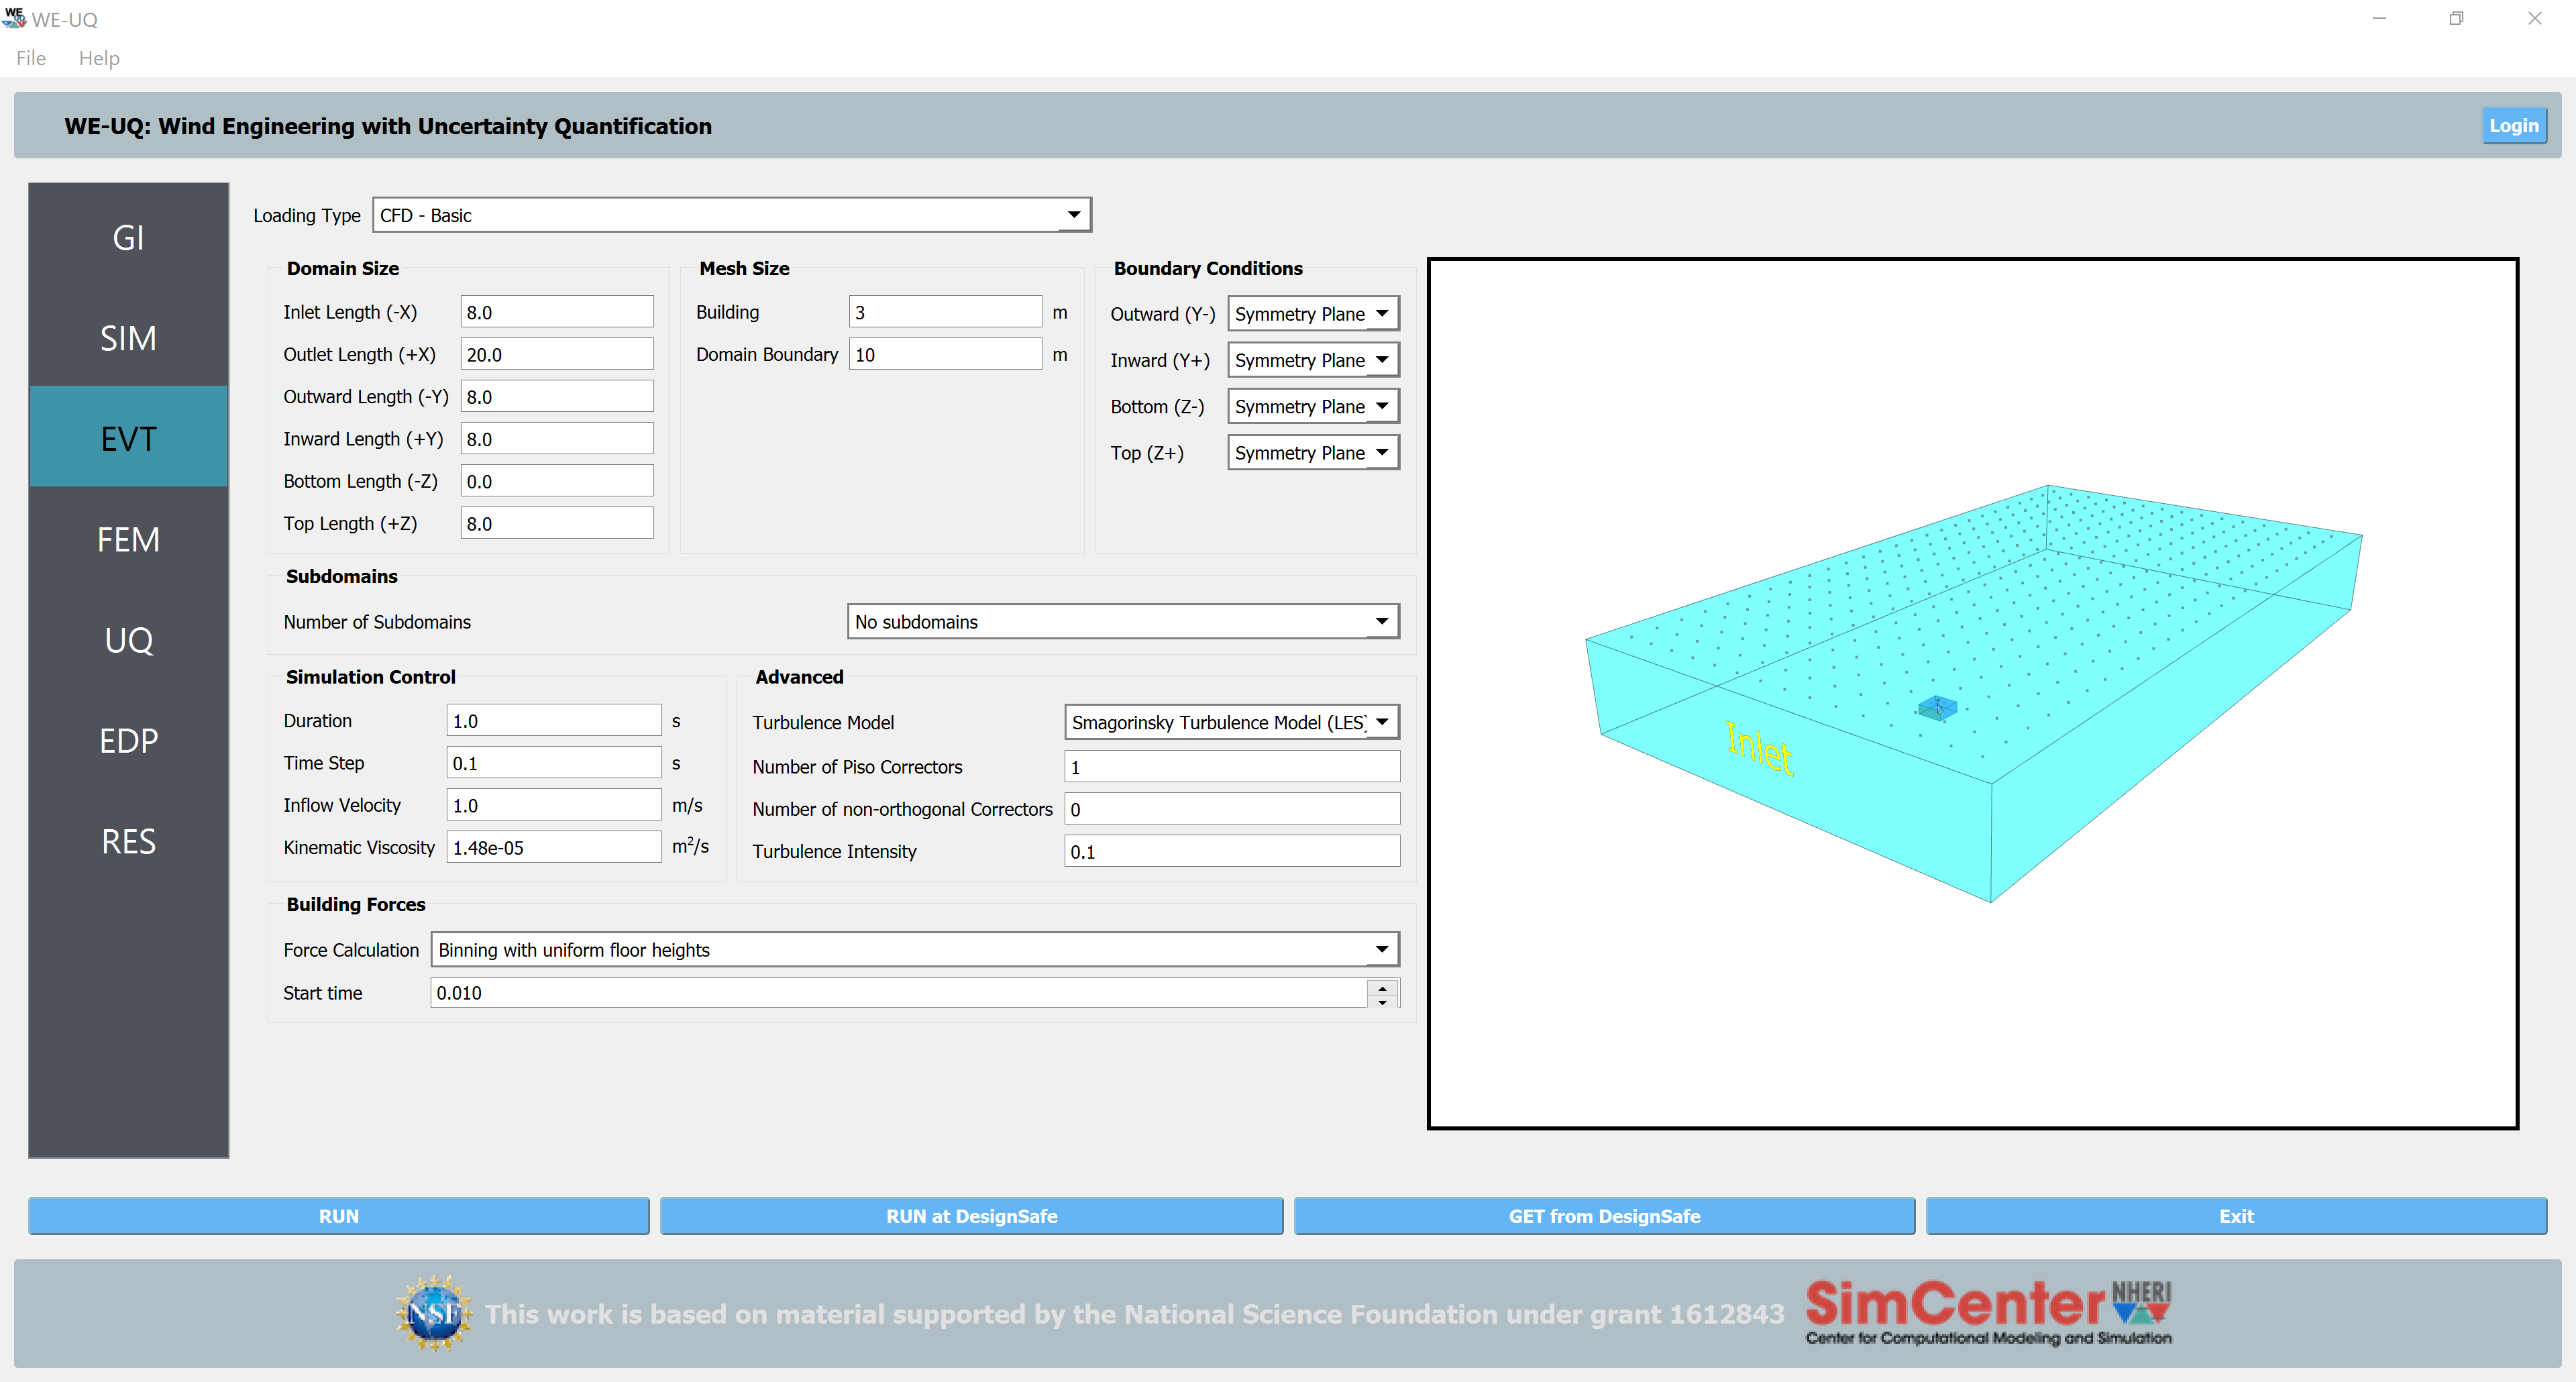
\includegraphics[width=0.95\textwidth]
        {usage/figures/cfd_template.png} }
    \caption{CFD Template Event}
    \label{fig:cfd_template}
\end{figure}

The following are the steps the user should follow to use the CFD template:

\begin{enumerate}
\item Specify the domain size in different directions using the input fields in the domain size group. It is important to note here that the size is relative to the building size. A three dimensional view is provided to allow the user to visualize the domain size. The 3D view should also indicate the location of the wind flow inlet.

\item Prescribe mesh sizes at the building surface and the outer edge of the wind field boundary. Mesh sizes are specified in meters. Users can visualize the prescribed mesh size compared to the domain and building sizes, only for the top surfaces.

\item The next step is to specify the boundary conditions on the sides, top and bottom of the domain. The user can select between wall or symmetry plane boundary conditions.

\item Optionally, the user can also specify up to three inner sub-domains. The desired mesh size and dimensions of sub-domains can be specified and they follow the same convention as the main domain.

\item Basic and advanced simulation parameters needs to be specified. The user can specify the total time, time step, wind velocity, turbulence model used in the OpenFOAM CFD simulation.

\item  Finally, the user needs to specify how the force on the building are extracted. Currently, the only method supported is to group forces on the building into bins of equal height, where each bin corresponds to a building floor. In addition, a start time for the applying the forces on the building model has to be specified, forces before that time will not be used. This allows the user to ignore force values in the beginning of the CFD simulation as they may not be accurate.

\end{enumerate}

It has to be noted that this event can only run remotely at DesignSafe-CI, and is not supported to be run on the local computer. Once the analysis is run a mesh is generated using Gmsh based on the meshing parameters specified by the user, then and OpenFOAM model is generated, analyzed and its output will be used to extract forces acting on the building, assuming the building is a rigid body. It is also important to note that intermediate meshing and CFD simulation results are available in the output archive folder for the user to inspect, if needed. 
